\chapter{Magnetic Field and Magnetic Forces}
So far we have discussed electric fields $\vec{E}$, which give force $\vec{F}_E = q \vec{E}$ on a charge $q$, no matter what its velocity. But the electromagnetic field also includes another vector field, the magnetic field $\vec{B}$, which gives a force $\vec{F}_B = q\vec{v} \times \vec{B}$ on a charge $q$ that depends on its velocity $\vec{v}$ and is zero if the velocity is zero. 

The magnitude of the magnetic force is 
\begin{equation}
F_B = \abs{\vec{F}_B} = \abs{q\vec{v}\times \vec{B}} = \abs{q}v_\perp B = \abs{q}vB \sin \theta,
\end{equation}
where $v_\perp = v \sin \theta$ is the component of the velocity perpendicular to $\vec{B}$. $\vec{F}_B$ is perpendicular to both $\vec{v}$ and $\vec{B}$ and with the sense that one's right thumb would point if one's fingers coiled from first being in the direction of $\vec{v}$ and then towards the tips in the $\vec{B}$ direction. 

\begin{wrapfigure}{R}{5cm}
\centering
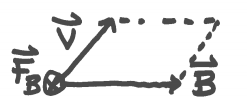
\includegraphics[width=5cm]{Images/chap7_1.png}
\end{wrapfigure}

$\vec{v} \times \vec{B}$ has magnitude $\vec{v}$ and $\vec{B}$. It is the vector `area' $\vec{A} = \vec{v} \times \vec{B}$ associated with this parallelogram, perpendicular to the area itself. In this case the vector $\vec{v} \times \vec{B}$ points into the page (or screen when the image is projected), as indicated by $\otimes$, which symbolizes the tail feathers of an arrow pointing away. The opposite arrow perpendicular to the paper, say $-\vec{v} \times \vec{B} = \vec{B} \times \vec{v}$, would be indicated by $\odot$, which symbolizes the tip of an arrow pointing toward the viewer.

The sense can also be given by the direction the tip of a screw would move if it's axis were perpendicular to $\vec{v}$ and $\vec{B}$ and its head (parallel to the plane of $\vec{v}$ and $\vec{B}$) were turned by $<180\deg$ from $\vec{v}$ to $\vec{B}$.

When both an electric field $\vec{E}$ and a magnetic field $\vec{B}$ is present, the total electromagnetic field force on a particle of charge $q$ and velocity $\vec{v}$ is called the \textbf{Lorentz force},
\begin{equation}
\boxed{\vec{F} = q(\vec{E} + \vec{v} \times \vec{B})}.
\end{equation}

Electric fields are produced by charges whether or not they are moving (though the electric fields deviate from Coulomb's law if the charges are accelerating or have velocities comparable to the speed of light, $\SI{299792456}{\frac{m}{s}}$), but magnetic fields are produced only by charges that are moving and/or accelerating. Later we shall discuss the analogues of Coulomb's law for how magnetic fields are produced. Charges moving within atoms and molecules are one way. Another is that even a charge not moving can have a spin, which produce a dipole magnetic field.

Just as the electric field $\vec{E}$ has electric field lines that are everywhere parallel to $\vec{E}$ and that give a flux $\Phi_E = \oint \vec{E} \cdot \di \vec{A}$ through a surface, so a magnetic field $\vec{B}$ has \textbf{magnetic field lines} everywhere parallel to $\vec{B}$ and that give a flux $\Phi_B = \int \vec{B} \cdot \di \vec{A}$ through a surface. For the electric field, Gauss's law gives the electric flux outward through a closed surface as 
\begin{equation}
\Phi_E = \oint \vec{E} \cdot \di \vec{A} = \frac{Q_{encl}}{\varepsilon_0},
\end{equation}
where $Q_{encl}$ is the total electric charge inside the volume enclosed by the surface. The analogue for the magnetic field would be $\Phi_B = \oint \vec{B} \cdot \di \vec{A} \propto$ (magnetic charge $Q_B$ enclosed). However, no magnetic charge $Q_B$ has ever been observed, so we shall say Gauss's law for magnetism is $\boxed{\oint \vec{B} \cdot \di \vec{A} = 0}$ through any closed surface.

Analogous to the way that Maxwell in 1865 completed the development of \textbf{electromagnetism} started by Coulomb, Gauss, Ampere, Faraday, and others, the 1960s saw the unification of electromagnetism and the \textbf{weak interaction} (radioactivity) by Glashow, Weinberg, and Salam. When combined with the theory of \textbf{quantum chromodynamics} for the strong nuclear reactions, including the Higgs mechanism for generating the masses of quarks (the building blocks for hadrons such as protons and neutrons) and of electrons and related other leptons, this gives what is known as the \textbf{Standard Model} of particle physics. However, this treats rather separately, and does not fully unify, the \textbf{electroweak} and \textbf{strong} interactions. Such a unification would be a \textbf{Grand Unified Theory}.

Such a \textbf{Grand Unified Theory} (GUT) would explain why the electron charge seems to be exactly the same magnitude (but opposite sign) as the proton charge, and, related to this, it predicts the existence of \textbf{magnetic monopoles}, which would have nonzero magnetic charge. However, these magnetic monopoles are predicted to have energies about a trillion times larger than the energies that can be produced in the largest accelerator today, the \textbf{Large Hadronic Collider (LHC)} at CERN, where several UofA professors work. So unless these estimates are wrong, it might be too difficult for humans ever to produce magnetic monopoles. Therefore, in this course we shall assume $\oint \vec{B} \cdot \di \vec{A} = 0$ or no magnetic monopoles.

\textbf{Gauss's Law for magnetism with no magnetic monopoles}, or $\boxed{\oint \vec{B} \cdot \di \vec{A} = 0}$, implies that magnetic field lines have no beginning or end. Generally, they come in from infinity and go back out to infinity, but they can also wrap around and around in a finite volume without ever reconnecting, unlike what the textbook says near the bottom of p.889: ``Like all other magnetic field lines, they form closed loops." Only in special situations, such as symmetry of rotation about an axis, or other situations in which a set of field lines stay in one plane without going to infinity, do the field lines form closed loops.

Asymmetric field lines do not stay on any single non-branching surface, and they need not form closed loops. A permanent magnet longer along the direction of the magnetic field inside has a north pole end (N) and a south pole end (S). Magnetic field lines run through the magnet from the S end to the N end and then emerge to loop back outside (though) they need not stay in a plane or distorted plane to reconnect precisely). However, because magnetic field lines nowhere begin or end, if one cuts the magnet in two, one will not get an isolated north pole or south pole, but rather the two new magnets will each have a north pole end and a south pole end, with the magnetic field passing through each magnet from south to north and then looping back outside, without ever ending.

A compass needle is a magnet free to rotate in the horizontal plane (when the compass is level), and then the north pole end of the compass points in the direction of the horizontal component of the magnetic field. From a Natural Resources Canada magnetic declination calculator online, when I entered the date 2019 March 12 and latitude $\frac{\pi}{2} - \frac{2}{\pi}$ radians = $\ang{53.5244}$N and longitude $\frac{5\pi}{6} - \frac{2}{\pi}$ radians = $\ang{113.5244}$W for the University of Alberta (``colatitude equator's reciprocal", and longitude $\pi/3 = \ang{60}$ greater than latitude), 1 got a magnetic declination of $\ang{14.094}$E, meaning that a compass would point $\ang{14.094}$ east of true north. It also said that this declination is decreasing about $\ang{1.04}$ every 6 years. Where I lived in Manokotak, Alaska, the declination decreased from $\ang{20}$E when I first went there in late summer 1959 to $\ang{12.2}$E today, a decreased of $\ang{7.8}$ in 60 years, an average decrease of $\ang{0.13}$/year or $\ang{1}$/(8 years).

The earth itself acts like a relatively permanent magnet, though its magnetic field is gradually changing with time (for example, with the North Magnetic Pole, where $\vec{B}$ is vertically downward, moving across northern Canadian islands during my lifetime, now being north of the Canadian Arctic territorial claim and within $\ang{4}$ of the Geographic North Pole and moving toward Russia at 55-60 km/year) and also reverses at random time intervals ranging between 100000 years and 50000000 years, the most recent being about 780000 years ago.

The earth's magnetic field is crudely a dipole field, with the dipole part having an axis that passes through the North Geomagnetic Pole that in 2015 was located at $\ang{80.37}$N, on Ellesmere Island, Nunavut, Canada. But because the field is not purely a dipole, the North Magnetic Pole and the North Geomagnetic Pole do not coincide, and a compass needle does not point to either.

When two magnets are placed close together end to end, the magnetic field energy is lower if the magnetic field on the axis is aligned: $\boxed{\text{S} \rightarrow \text{N}}$  $\boxed{\text{S} \rightarrow \text{N}}$ Thus the north pole of one magnet attracts the south pole of another, so opposite poles attract, rather similar to the way opposite charges attract and charges of the same sign repel, except that for magnets, one cannot have isolated poles. But since the north pole of a compass is attracted towards the north magnetic pole of the earth (where the magnetic field enters the earth vertically downwards), if one views the earth as a magnet, the North Magnetic Pole, or perhaps slightly better, the North Geomagnetic Pole (intersection of the dipole axis with the earth in the north), is a magnetic south pole, where magnetic field lines enter the earth, as they do in the south pole of a magnet.

Since the magnetic force magnitude is
\begin{equation}
F_B = \abs{\vec{F}_B} = \abs{q \vec{v} \times \vec{B}} = \abs{q} v_\perp B = \abs{q} v B_\perp ,
\end{equation}
the units of magnetic field are those of $\frac{F}{qv} = \SI{}{\frac{kg \cdot m/s^2}{C \cdot m/s} = \SI{}{\frac{kg}{C \cdot s}} = \SI{}{\frac{kg}{A \cdot s^2}} = \SI{}{T}}$, the \textbf{tesla}, (in honor of Nikola Tesla, 1856-1943, the prominent Serbian-American scientist and inventor). $\SI{1}{T} = \SI{1}{\frac{kg}{A \cdot s^2}} = \SI{1}{\frac{N}{A \cdot m}}$. 

Another common unit is the \textbf{gauss (G)}, $\SI{1}{G} = \SI{e-4}{T}$, a more convenient unit for the earth's magnetic field, since over the earth's surface, $B$ ranges from $\SI{0.25}{G}$ to $\SI{0.65}{G}$. For Edmonton 2019 March 12, $B = \SI{0.56797}{G}$, with an inclination angle of $\ang{75.096}$, a vertical component of $\SI{0.54886}{G}$ downward, a horizontal component of $\SI{0.54886}{G}$ $\ang{14.094}$ E of north, given a northward component of $\SI{0.14169}{G}$ and an eastward component of $\SI{0.03557}{G}$.

I tried to get a crude estimate for the magnetic flux outward through the part of the earth's surface where the outward radial (locally vertical) component $B_r$ of the magnetic field is positive (mainly in the southern hemisphere, south of what might call the `magnetic equator'), where the magnetic field has $B_r = 0$ and is parallel to the earth's surface, by which 1 mean the surface if the \textbf{geoid} which is the gravitational equipotential surface at mean sea level in the rotating frame of the earth, the rotation causing the geoid to be approximately ellipsoidal, and in fact given by a nominal ellipsoid to first approximation that has been chosen to have a semi-major axis $a = \SI{6378137}{m}$ and a semi-minor axis $b=a(1-1/298257223563)$.

A dipole approximation for the field gives
\begin{equation}
B_r = -2B_o\pfrac{R_\oplus}{r}^3 \cos \theta,
\end{equation}
where $\theta$ is the angle from the north end of the dipole axis and $B_o = \SI{3.12e-5}{T}$ is the value of the dipole field at $\theta = \frac{\pi}{2}$, where it is purely tangential (parallel to the sphere at that value of $r$). Then since a narrow band on a sphere of radius $r = R_\oplus =$ earth's radius of angular width $\di \theta$ has width $r \di \theta$ and length $2 \pi r \sin \theta$, its area is $\di A = 2 \pi r^2 \sin \theta \di \theta$. This gives the total area of the sphere as